% !TEX ROOT = ersti.tex
\section{Ansprechpartner im Studium}

Nicht nur am Anfang eures Studiums, sondern auch mitten drin, können kleinere und
größere Fragen und Probleme auftreten. Damit ihr mit diesen Problemen nicht alleine
da steht, gibt es mehrere Personen, die euch bei diesen helfen können. Erster
Ansprechpartner in allen Dingen ist natürlich die Fachschaft (siehe dazu Artikel
über die Fachschaft). Falls wir euch dann nicht weiter helfen können, gibt es an
jeder Fakultät noch weitere Ansprechpartner.

\newcommand{\proffoto}[2]{
    \centering
    \includegraphics[width=3cm]{#1}\\
    #2
    \vspace{4mm}
}

\begin{description}
\sidebar{
    \chaptersidebarpushdown
    \ifdefined\dekanphysikfoto
    \proffoto{\dekanphysikfoto}{\dekanphysiklang\\[-1ex]{\scriptsize Dekan Physik}}
    \fi

    \ifdefined\dekanmathefoto
    \proffoto{\dekanmathefoto}{\dekanmathelang\\[-1ex]{\scriptsize Dekan Mathe}}
    \fi

    \ifdefined\studiendekaninformatikfoto
    \proffoto{\studiendekaninformatikfoto}{\studiendekaninformatik\\[-1ex]{\scriptsize Studiendekanin Info}}
    \fi

    \ifdefined\studiendekanphysikfoto
    \proffoto{\studiendekanphysikfoto}{\studiendekanphysik\\[-1ex]{\scriptsize Studiendekan Physik}}
    \fi

    \vspace*{1.8cm}

    \ifdefined\studiendekanmathefoto
    \proffoto{\studiendekanmathefoto}{\studiendekanmathe\\[-1ex]{\scriptsize Studiendekan Mathe}}
    \fi

    \ifdefined\prodekanphyikfoto
    \proffoto{\prodekanphyikfoto}{\prodekanphysik\\[-1ex]{\scriptsize Prodekan Physik}}
    \fi

    % Rest weiter unten weil die Physik zwei Prodekane hat
    % und damit nicht mehr alles in die Spalten passt
}

\item[Der Dekan] ist sozusagen ChefIn der Fakultät und leitet diese. Er wird
	für vier Jahre gewählt. In der Mathe \& Informatik ist \dekanmathelang\
	Dekan, in der Physik \dekanphysiklang .

\item[Der Prodekan] ist VertreterIn des Dekans und unterstützt diesen in seinen
	Aufgaben. In der Mathe \& Informatik ist \prodekanmathe\ Prodekan, in der
	Physik \prodekanphysik .

\item[Das Dekanat] ist das Sekretariat der Fakultät. Hier kann euch geholfen
	werden, wenn ihr nicht wisst, an wen ihr euch genau wenden sollt. (In der
	Mathe: Tel.  \dekanatmathetelefon , in der Physik: Tel.
	\dekanatphysiktelefon )

\item[Der Studiendekan] ist Vorsitzender der Studienkommission. Diese ist für
	alle Fragen der Lehre zuständig und auch die erste Adresse bei Fragen und
	Problemen. In der Mathe ist \studiendekanmathe\ Studiendekan, in der
	Informatik \studiendekaninformatik , in der Physik \studiendekanphysik .

\item[Die Studienberatung] Fragen zur persönlichen Studienplanung, zur
	Orientierung und zur allgemeinen Beratung beantworten in jeder Fakultät
	eigens abgestellte Studienberater. So zum Beispiel \studienberatungmathe\
	in der Mathe, \studienberatunginformatik\ in der Informatik und
	\studienberatungphysik\ in der Physik.

\item[Deine Fachschaft] vertritt die Interessen der Studierenden in den
	Fakultätsgremien und ist diskreter Ansprechpartner bei Problemen mit einem
	Dozenten oder Fragen zur Prüfungsordnung. \\\fsraum;
	\url{fachschaft@mathphys.fsk.uni-heidelberg.de}

\item[Das Prüfungssekretariat] ist zuständig für Prüfungsfragen aller Art. Ob
	es jetzt um die Anrechnung von Modulen anderer Fakultäten, die Anmeldung
	von Bachelor-Arbeiten oder sonstige Fragen rund um die Prüfungsordnung
	geht, im Prüfungssekretariat sitzen kompetente Menschen, die dir
	weiterhelfen. In der Informatik ist das \pruefsekinfo, in der Mathe
	\pruefsekmathe, in der Physik \pruefsekphysik.

\item[BAföG-Beauftragter] Spätestens zu Beginn des 5. Semesters braucht ihr
	einen Leistungsnachweis, dass ihr die bei geordnetem Verlauf der Ausbildung
	bis zum Ende des 4. Fachsemesters üblichen Leistungen erbracht habt. Dies
	bestätigt Euch in der Mathe \bafogmathe , in der Informatik
	\bafoginformatik\ und in der Physik \bafogphysik .

\item[Lehramt] Alle Fragen, die das Lehramt betreffen, können euch im Zentrum
	für Lehrerbildung beantwortet werden: ZLB, Akademiestr. 3 Zimmer 237

\item[Gleichstellungskommissionen] setzen sich für die Chancengleichheit von
	Frauen und Männern ein und informieren über gesetzliche Regelungen. Falls
	ihr Fragen zum Thema Gleichstellung habt, könnt ihr euch jederzeit an sie
	wenden. Gleichstellungsbeauftragte in der Physik ist
	\frauenbeauftragtephysik\ (\url{gleichstellung@lsw.uni-heidelberg.de}), in
	der Mathe \& Informatik \frauenbeauftragtemathe .


\end{description}


\noindent Die Zuständigen für die jeweiligen Bereiche wechseln gelegentlich, können aber immer
aktuell auf den Internetseiten der entsprechenden Fakultäten eingesehen werden. Dort
findet ihr auch alle Sprechzeiten und Telefonnummern. Achtung: manchmal ist auch
eine vorherige Anmeldung erforderlich! Oft kann man die DozentInnen aber auch
außerhalb ihrer Sprechzeiten erreichen, zur Not immer per E-Mail.\\[.9cm]

\relax

% Hinweis zu den Abständen:
% die 1.3cm oben sind von Hand abgemessen, sodass der Abstand zwischen
% den Fotos in der Sidebar hier fortgesetzt wird
% die -5.52cm sind von Hand abgemessen, sodass die Fotos links bündig
% sind (bzw. die -1.695cm rechtsbündig für ungerade Seiten)
% die 1.51\textwidth sind auch von Hand abgemessen, sodass das Foto
% bzw. die Fotounterschrift (je nach dem was länger ist) rechts mit dem
% Text oben drüber bündig wird
% Alle Fotos sind 4 cm breit. Die Fotos in sollten alle das gleiche
% Seitenverhältnis (BxH: 200x267 bzw. wer Lust hat darf das kürzen)
% haben, wenn man unschöne Effekte vermeiden will
\iftrue
\checkoddpage
\ifoddpage
    %\hspace*{-1.695cm}
    \hspace*{-1.15cm}
\else
    \hspace*{-5.52cm}
\fi
\begin{minipage}{1.51\textwidth}
\parbox [t]{0.3\textwidth}{
    \ifdefined\prodekanmathefoto
    \proffoto{\prodekanmathefoto}{\prodekanmathe\\[-1ex]{\scriptsize Prodekan Mathe}}
    \fi
}
\hfill
\parbox[t]{0.3\textwidth}{
    \ifdefined\prodekanphysikfotoA
    \proffoto{\prodekanphysikfotoA}{\prodekanphysikA\\[-1ex]{\scriptsize Prodekan Physik}}
    \fi
}
\hfill
\parbox [t]{0.3\textwidth}{
    \ifdefined\prodekanphysikfotoB
    \proffoto{\prodekanphysikfotoB}{\prodekanphysikB\\[-1ex]{\scriptsize Prodekan Physik}}
    \fi
}
\end{minipage}
\else
\checkoddpage
\ifoddpage
    \hspace*{-1.695cm}
    %\hspace*{-1.15cm}
\else
    %\hspace*{-5.52cm}
    \hspace*{-4.55cm}
\fi
\begin{minipage}{1.51\textwidth}
%\hfill
\parbox [t]{0.24\textwidth}{
    \ifdefined\prodekanmathefoto
    \proffoto{\prodekanmathefoto}{\prodekanmathe\\[-1ex]{\scriptsize Prodekan Mathe}}
    \fi
}
\hfill
\parbox[t]{0.24\textwidth}{
    \ifdefined\prodekanphysikfotoA
    \proffoto{\prodekanphysikfotoA}{\prodekanphysikA\\[-1ex]{\scriptsize Prodekan Physik}}
    \fi
}
\hfill
\parbox [t]{0.24\textwidth}{
    \ifdefined\prodekanphysikfotoB
    \proffoto{\prodekanphysikfotoB}{\prodekanphysikB\\[-1ex]{\scriptsize Prodekan Physik}}
    \fi
}
\hfill
\parbox [t]{0.24\textwidth}{
    \ifdefined\studiendekanmathefoto
    \proffoto{\studiendekanmathefoto}{\studiendekanmathe\\[-1ex]{\scriptsize Studiendekan Mathe}}
    \fi
}
\end{minipage}
\fi

% Wenn noch Platz ist, z.B. weil Fotos fehlen oder die Physik
% nur noch einen Prodekan hat, kann man das als Lückenfüller nehmen:

%~ \begin{figure}[h]
%~ \vspace{10mm}
%~ \centering{
    %~ 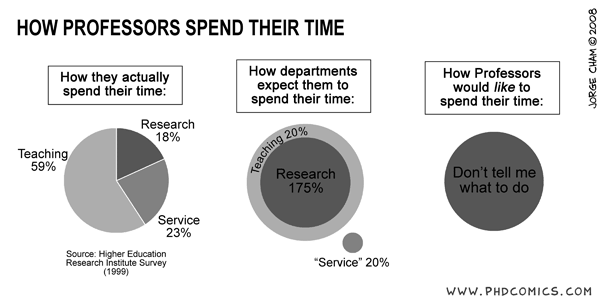
\includegraphics[width=\textwidth]{bilder/Prof.png}
%~ }
%~ \end{figure}



